% Options for packages loaded elsewhere
\PassOptionsToPackage{unicode}{hyperref}
\PassOptionsToPackage{hyphens}{url}
%
\documentclass[
  12pt,
  a4paper,
  openany]{book}
\usepackage{lmodern}
\usepackage{setspace}
\usepackage{amssymb,amsmath}
\usepackage{ifxetex,ifluatex}
\ifnum 0\ifxetex 1\fi\ifluatex 1\fi=0 % if pdftex
  \usepackage[T1]{fontenc}
  \usepackage[utf8]{inputenc}
  \usepackage{textcomp} % provide euro and other symbols
\else % if luatex or xetex
  \usepackage{unicode-math}
  \defaultfontfeatures{Scale=MatchLowercase}
  \defaultfontfeatures[\rmfamily]{Ligatures=TeX,Scale=1}
  \setmainfont[]{Arial}
\fi
% Use upquote if available, for straight quotes in verbatim environments
\IfFileExists{upquote.sty}{\usepackage{upquote}}{}
\IfFileExists{microtype.sty}{% use microtype if available
  \usepackage[]{microtype}
  \UseMicrotypeSet[protrusion]{basicmath} % disable protrusion for tt fonts
}{}
\usepackage{xcolor}
\IfFileExists{xurl.sty}{\usepackage{xurl}}{} % add URL line breaks if available
\IfFileExists{bookmark.sty}{\usepackage{bookmark}}{\usepackage{hyperref}}
\hypersetup{
  hidelinks,
  pdfcreator={LaTeX via pandoc}}
\urlstyle{same} % disable monospaced font for URLs
\usepackage[left=3.5cm,right=2cm,top=3cm,bottom=3cm, asymmetric]{geometry}
\usepackage{color}
\usepackage{fancyvrb}
\newcommand{\VerbBar}{|}
\newcommand{\VERB}{\Verb[commandchars=\\\{\}]}
\DefineVerbatimEnvironment{Highlighting}{Verbatim}{commandchars=\\\{\}}
% Add ',fontsize=\small' for more characters per line
\usepackage{framed}
\definecolor{shadecolor}{RGB}{248,248,248}
\newenvironment{Shaded}{\begin{snugshade}}{\end{snugshade}}
\newcommand{\AlertTok}[1]{\textcolor[rgb]{0.94,0.16,0.16}{#1}}
\newcommand{\AnnotationTok}[1]{\textcolor[rgb]{0.56,0.35,0.01}{\textbf{\textit{#1}}}}
\newcommand{\AttributeTok}[1]{\textcolor[rgb]{0.77,0.63,0.00}{#1}}
\newcommand{\BaseNTok}[1]{\textcolor[rgb]{0.00,0.00,0.81}{#1}}
\newcommand{\BuiltInTok}[1]{#1}
\newcommand{\CharTok}[1]{\textcolor[rgb]{0.31,0.60,0.02}{#1}}
\newcommand{\CommentTok}[1]{\textcolor[rgb]{0.56,0.35,0.01}{\textit{#1}}}
\newcommand{\CommentVarTok}[1]{\textcolor[rgb]{0.56,0.35,0.01}{\textbf{\textit{#1}}}}
\newcommand{\ConstantTok}[1]{\textcolor[rgb]{0.00,0.00,0.00}{#1}}
\newcommand{\ControlFlowTok}[1]{\textcolor[rgb]{0.13,0.29,0.53}{\textbf{#1}}}
\newcommand{\DataTypeTok}[1]{\textcolor[rgb]{0.13,0.29,0.53}{#1}}
\newcommand{\DecValTok}[1]{\textcolor[rgb]{0.00,0.00,0.81}{#1}}
\newcommand{\DocumentationTok}[1]{\textcolor[rgb]{0.56,0.35,0.01}{\textbf{\textit{#1}}}}
\newcommand{\ErrorTok}[1]{\textcolor[rgb]{0.64,0.00,0.00}{\textbf{#1}}}
\newcommand{\ExtensionTok}[1]{#1}
\newcommand{\FloatTok}[1]{\textcolor[rgb]{0.00,0.00,0.81}{#1}}
\newcommand{\FunctionTok}[1]{\textcolor[rgb]{0.00,0.00,0.00}{#1}}
\newcommand{\ImportTok}[1]{#1}
\newcommand{\InformationTok}[1]{\textcolor[rgb]{0.56,0.35,0.01}{\textbf{\textit{#1}}}}
\newcommand{\KeywordTok}[1]{\textcolor[rgb]{0.13,0.29,0.53}{\textbf{#1}}}
\newcommand{\NormalTok}[1]{#1}
\newcommand{\OperatorTok}[1]{\textcolor[rgb]{0.81,0.36,0.00}{\textbf{#1}}}
\newcommand{\OtherTok}[1]{\textcolor[rgb]{0.56,0.35,0.01}{#1}}
\newcommand{\PreprocessorTok}[1]{\textcolor[rgb]{0.56,0.35,0.01}{\textit{#1}}}
\newcommand{\RegionMarkerTok}[1]{#1}
\newcommand{\SpecialCharTok}[1]{\textcolor[rgb]{0.00,0.00,0.00}{#1}}
\newcommand{\SpecialStringTok}[1]{\textcolor[rgb]{0.31,0.60,0.02}{#1}}
\newcommand{\StringTok}[1]{\textcolor[rgb]{0.31,0.60,0.02}{#1}}
\newcommand{\VariableTok}[1]{\textcolor[rgb]{0.00,0.00,0.00}{#1}}
\newcommand{\VerbatimStringTok}[1]{\textcolor[rgb]{0.31,0.60,0.02}{#1}}
\newcommand{\WarningTok}[1]{\textcolor[rgb]{0.56,0.35,0.01}{\textbf{\textit{#1}}}}
\usepackage{longtable,booktabs}
% Correct order of tables after \paragraph or \subparagraph
\usepackage{etoolbox}
\makeatletter
\patchcmd\longtable{\par}{\if@noskipsec\mbox{}\fi\par}{}{}
\makeatother
% Allow footnotes in longtable head/foot
\IfFileExists{footnotehyper.sty}{\usepackage{footnotehyper}}{\usepackage{footnote}}
\makesavenoteenv{longtable}
\usepackage{graphicx}
\makeatletter
\def\maxwidth{\ifdim\Gin@nat@width>\linewidth\linewidth\else\Gin@nat@width\fi}
\def\maxheight{\ifdim\Gin@nat@height>\textheight\textheight\else\Gin@nat@height\fi}
\makeatother
% Scale images if necessary, so that they will not overflow the page
% margins by default, and it is still possible to overwrite the defaults
% using explicit options in \includegraphics[width, height, ...]{}
\setkeys{Gin}{width=\maxwidth,height=\maxheight,keepaspectratio}
% Set default figure placement to htbp
\makeatletter
\def\fps@figure{htbp}
\makeatother
\setlength{\emergencystretch}{3em} % prevent overfull lines
\providecommand{\tightlist}{%
  \setlength{\itemsep}{0pt}\setlength{\parskip}{0pt}}
\setcounter{secnumdepth}{5}
\pagestyle{plain}
\usepackage{booktabs}
\usepackage{amsmath,amsfonts,amsthm,bm} % Math packages
\usepackage{mathtools, cases}
\usepackage{fontspec}
\usepackage[utf8]{inputenc}
\usepackage[portuguese]{babel}

\usepackage{etoolbox}

\usepackage{ragged2e}

\usepackage{titlesec}

\usepackage{graphicx}
\usepackage{placeins}

\usepackage{makeidx}
\makeindex
\usepackage[nottoc]{tocbibind}

\makeatletter
\patchcmd{\ttl@save@mkschap}{*}{}{}{}
\makeatother
\usepackage{indentfirst}
\usepackage{floatrow}
\floatsetup[figure]{capposition=top}
\floatsetup[table]{capposition=top}
\usepackage{subfig}
\usepackage{booktabs}
\usepackage{longtable}
\usepackage{array}
\usepackage{multirow}
\usepackage{wrapfig}
\usepackage{float}
\usepackage{colortbl}
\usepackage{pdflscape}
\usepackage{tabu}
\usepackage{threeparttable}
\usepackage{threeparttablex}
\usepackage[normalem]{ulem}
\usepackage{makecell}
\usepackage{xcolor}
\ifluatex
  \usepackage{selnolig}  % disable illegal ligatures
\fi
\usepackage[]{natbib}
\bibliographystyle{apalike}

\author{}
\date{\vspace{-2.5em}}

\begin{document}

%titlepage
\thispagestyle{empty}
\begin{center}
\begin{minipage}{0.90\linewidth}
    \centering
%University logo
    
\includegraphics[width=1\textwidth]{image/biglogo.png}

%Thesis title
    {\uppercase{\Large Impacto da volatilidade na otimização de portfolios financeiros\par}}
    \vspace{2cm}
%Author's name
    {\Large Leonel da Silva Baptista\par}
    \vspace{2cm}
%Degree
    {\Large Mestrado em Estatística, Matemática e Computação\par}
    {\Large Ramo Estatística Computacional\par}
    \vspace{2cm}

%Date
    {\Large 2020}
\end{minipage}
\end{center}


%titlepage
\thispagestyle{empty}
\begin{center}
\begin{minipage}{0.90\linewidth}
    \centering
%University logo
    
\includegraphics[width=1\textwidth]{image/logo.png}

%Thesis title
    {\uppercase{\Large Impacto da volatilidade na otimização de portfolios financeiros\par}}
    \vspace{2cm}
%Author's name
    {\Large Leonel da Silva Baptista\par}
    \vspace{2cm}
%Degree
    {\Large Mestrado em Estatística, Matemática e Computação\par}
    {\Large Ramo Estatística Computacional\par}
    \vspace{2cm}
%oriented
    {\Large Dissertação orientada pelo\par}
    {\Large Professor Doutor Amílcar Manuel do Rosário Oliveira\par}
    \vspace{2cm}
%Date
    {\Large 2020}
\end{minipage}
\end{center}

\pagenumbering{gobble}% Remove page numbers (and reset to 1)

\clearpage

\chapter*{Resumo}
\fontsize{12}{21}\selectfont
A presente dissertação têm como âmbito a análise de três métodos diferentes de obter a volatilidade de instrumentos financeiros, nomeadamente valores mobiliários, e seu consequente impacto no resultado da rentabilidade de portfolios constituídos utilizando como pressuposto a média variância, assim como a sua exposição ao risco, sendo que a volatilidade constitui uma peça central na constituição de determinados instrumentos financeiros e respetivo calculo de exposição ao risco.

Os métodos analisados para calculo da volatilidade são a Média Movel Exponencial (EWMA), o modelo da heteroscedasticidade condicional auto-regressiva generalizada (GARCH) e a volatilidade implícita. Os dois primeiros métodos têm como subjacentes dados históricos dos instrumentos financeiros, sendo que a volatilidade implícita é a volatilidade esperada pelo mercado, sendo obtida através da cotação das opções dos respetivos subjacentes.

A análise de risco é efetuada aplicando dois métodos complementares de análise. O Value at Risk (VaR), que contempla a percentagem de perdas que excedem o VaR e o Expected shortfall (ES), que contempla a magnitude dessas perdas.

Este trabalho é realizado tendo como ferramenta de apoio a linguagem de programação R.
\bigbreak

\noindent\textbf{Palavras chave:} Volatilidade, portfolio, rentabilidade, risco, R




\pagenumbering{roman}% Arabic page numbers (and reset to 1)
\setcounter{page}{2}

\chapter*{Abstract}
\fontsize{12}{21}\selectfont
The scope of this dissertation is to analyze three different methods of obtaining the volatility of financial instruments, namely securities, and their consequent impact on the profitability of portfolios constituted using the assumption of mean-variance, as well as their exposure to risk, volatility is a central element in the constitution of certain financial instruments and the respective calculation of exposure to risk.

The methods analyzed for calculating the volatility are the Exponential Moving Average (EWMA), the generalized autoregressive conditional heteroscedasticity model (GARCH) and the implied volatility. The first two methods are based on historical data on financial instruments, the implied volatility being the volatility expected by the market, being obtained through the quotation of the options of the respective underlying.

The risk analysis is carried out using two complementary methods of analysis. Value at Risk (VaR), which includes the percentage of losses that exceed VaR and Expected shortfall (ES), which considers the magnitude of these losses.

This work is carried out using the R programming language as a support tool.

\bigbreak

\noindent\textbf{Keywords:} Volatility, portfolio, profitability, risk, R

\newenvironment{dedication}
  {\clearpage           % we want a new page
   \itshape             % the text is in italics
   \raggedleft          % flush to the right margin
  }
  {\par % end the paragraph
   \vspace{\stretch{3}} % space at bottom is three times that at the top
   \clearpage           % finish off the page
  }
\begin{dedication}
{\Large Dedicado a minha esposa\par}
\end{dedication}

\chapter*{Agradecimentos}

\renewcommand*\contentsname{Índice}
{
\setcounter{tocdepth}{2}
\tableofcontents
}
\listoftables
\listoffigures
\setstretch{1.5}
\hypertarget{simbologia-e-notauxe7uxf5es}{%
\chapter*{Simbologia e notações}\label{simbologia-e-notauxe7uxf5es}}
\addcontentsline{toc}{chapter}{Simbologia e notações}

\mainmatter

\hypertarget{intro}{%
\chapter*{Introdução}\label{intro}}
\addcontentsline{toc}{chapter}{Introdução}

A estatística aplicada ao sector financeiro têm sido pratica comum nas últimas décadas, sendo que a sua aplicação não se resume apenas a estatística descritiva, tendo vindo a beneficiar dos avanços verificados na aplicação de ferramentas estatísticas para analise preditiva dos dados, devido essencialmente aos avanços tecnológicos no hardware de equipamentos informáticos que permitem a aplicação de algoritmos mais complexos que de outro modo não seria possível utilizar, pelo menos em tempo útil.

Um dos sectores com grande aplicabilidade dos métodos matemáticos e estatísticos nas finanças é a analise quantitativa, sendo as principais áreas de aplicação a estruturação de derivados, gestão do risco, trading automático e gestão de investimentos.

Historicamente, a analise quantitativa iniciou-se em 1900 com Louis Jean-Baptiste Alphonse Bachelier, onde a sua tese de doutoramento forneceu um modelo para estipular o preço de opções considerando uma distribuição normal (\url{https://en.wikipedia.org/wiki/Quantitative_analysis_(finance)}).

Na década de 50, Harry Markowitz escreveu um artigo intitulado ``Portfolio Selection'' que viria a revolucionar o modo como selecionar uma carteira de instrumentos financeiros, aplicando princípios de correlação e variância de modo a constituir portfolios de ações , onde a ``fronteira eficiente'' representa portfolios que maximizam retornos de acordo com o risco assumido, providenciando modelos que demonstravam que só com a diversificação de investimentos é que se conseguiria atingir a eficiência, embora só bastante mais tarde esta teoria começa-se a ver a sua aplicabilidade nas instituições financeiras. A aplicabilidade de técnicas estatísticas fica saliente quando Markowitz estipula que ``para usar a regra da média-variância na seleção de ações devemos ter procedimentos para encontrar \(\mu_i\) e \(\sigma_{ij}\) razoáveis. Estes procedimentos, eu acredito, devem combinar técnicas estatísticas e julgamento prático do Homem'' \citep[pp.91]{Markowitz1952}. As limitações do modelo prendem-se com pressuposto que não representam exatamente a realidade, como o pressuposto de que os retornos das ações seguem uma distribuição normal, sendo que a distribuição dos retornos segue muitas vezes uma distribuição com curtose leptocúrtica, apresentando caudas pesadas e um pico superior ao da distribuição normal.

Na década de 60, Sharpe, Lintner and Mossin desenvolveram um modelo para equilíbrio de mercado, definido como \emph{Capital Asset Pricing Model} (CAPM), descrevendo a relação entre risco sistemático e o retorno esperado. O modelo pressupõe que, se todos os investidores contêm o mesmo portfolio, então, em equilíbrio esse deve ser o portfolio de mercado. De acordo com \citet{Sharpe1964}, em equilíbrio os preços dos ativos de capital foram ajustados de forma que o investidor consiga atingir qualquer ponto desejado ao longo da reta do mercado capital, ou \emph{capital market line} (CMP), pressupondo que o investidor siga uma estratégia de diversificação do investimento. O CMP pode ser utilizado de modo a otimizar um portfolio caso seja contemplado uma taxa de juro sem risco na sua estruturação, sendo o ponto tangente a curva denominada de fronteira eficiente.

Também na década de 60 foi apresentado pela primeira vez o modelo de Black-Scholes-Merton, fornecendo uma solução para valorizar opções europeias e outros derivados. O modelo assume que os preços têm uma distribuição lognormal e que a volatilidade é constante ao longo do tempo. A volatilidade que é assumida neste modelo é a volatilidade implícita da opção, ou seja, a volatilidade para o qual o valor dado pelo modelo Black-Scholes-Merton iguala o preço de mercado. Outros modelos foram desenvolvidos de modo a valorizar opções e outros derivados financeiros, entre eles a arvore binomial e simulação de Monte Carlo.

Os vários modelos apresentados têm como finalidade contribuir para uma decisão mais informada por parte do investidor, sendo que na generalidade o investidor irá optar pelo investimento que apresenta um maior retorno de acordo com o risco a que se dispõem estar exposto, tendo em consideração o seu perfil e expectativas.A escolha do portfólio é feita resolvendo um problema de otimização, no qual o risco do portfólio é minimizado sendo definido como retrição o valor desejado de retorno esperado. Desta forma é importante quantificar o risco. Existem vários modelos para quantificar o risco, ou seja quantificar a perda esperada de acordo com a hipótese de ocorrência de determinado cenário, sendo que 2 desses modelos para análise do risco são o \emph{Value at Risk} (VaR) e o \emph{Expected Shortfall}, também denominado \emph{Conditional Value at Risk} (CVaR). De acordo com \citet{HistVaR}, em 1922 no New York Stock Exchange já eram exigidos requisitos de capital a alguns dos seus membros, tendo na década de 50 Markowitz e Roy, separadamente, publicado metodos para quantificar o VaR, sendo ambos bastante similares e com a finalidade de quantificar o risco a que estaria exposto um portfolio. A necessidade de utilizar medidas de risco mais sofisticada tornou-se mais visível na década de 80 devido ao aparecimento de produtos mais complexos e ao aumento da volatilidade dos mercados, sendo que devido a regulamentação cada vez mais exigente, como o Basel III e Solvency II, as instituições financeiras e seguradoras devem implementar mecanismos de gestão de risco, sendo que os requisitos de capital são bastante mais exigentes desde a ocorrência da crise do subprime em 2007. De acordo com os acordos de Basel o VaR deve ser estimado diariamente utilizando o percentil 99\textsuperscript{th}.

Todos estes modelos têm tido aplicabilidade na análise quantitativa financeira, sendo que novos modelos foram sendo desenvolvidos ou apenas melhorados de modo a dar resposta à realidade verificada no mercado. Como podemos subentender uma das disciplinas fundamentais na definição destes modelos é o conhecimento de estatística e a sua aplicação prática, quer através de técnicas paramétricas, onde se assume um pressuposto forte de que os valores de uma variável têm uma distribuição normal, seja através de técnicas não paramétricas, onde não se assume que a distribuição dos valores de uma variável apresentam distribuição normal.

O trabalho desenvolvido ao longo desta tese, propõem-se analisar o impacto que poderá ter o método de calculo da volatilidade sobre a definição de um portfolio, o seu retorno esperado assim como quantificar o risco a que se estará exposto. Desde os primeiros trabalhos de \citet{Markowitz1952} acerca da otimização de portfolios que vários outros trabalhos foram desenvolvidos para constituição e otimização de portfolios, sendo que nesta dissertação se irá aplicar o método introduzido por \citet{Markowitz1952}, utilizando a teoria da média-variância para a constituição de um portfolio. O mesmo se poderá afirmar acerca do cálculo da exposição ao risco por um portfolio, sendo, no entanto, o VaR e o CVaR dois dos métodos mais utilizados para quantificar essa métrica, sendo que de acordo com \citet{OptVaR2000} o CVaR é conhecido por ter melhores propriedades que o VaR. Como iremos ver existem diferentes métodos de calculo do VaR e CVaR, sendo que neste trabalho iremos utilizar a que for mais adequada ao tipo de dados em análise.

Como inicialmente referido, o objetivo é analisar as diferentes formas de calcular a variância, sendo que iremos focar-nos em três formas diferentes de calcular esse valor, análisar a sua implicação no resultado final, assim como o valor que resulta da quantificação de risco e o seu impacto na perceção pelo investidor.

A investigação decorrerá aplicando-se os diferentes métodos de calculo da variância a dados do mercado, assim como os pressupostos teóricos de cada um dos métodos, sendo constituída uma carteira de ações integrantes do Euro Stoxx 50, calculando o seu retorno final para cada uma das volatilidades, assim como o risco a que está exposto um investidor. O retorno obtido será também comparado com um \emph{benchmark}, neste caso o Euro Stoxx 50.

Ao longo deste percurso será também análisada a forma como é constituídos um portfolio, a teoria subjacente a média-variância, as retrições aplicáveis ao modelo desenvolvido, assim como a teoria subjacente aos vários métodos para análise da exposição ao risco aquando da constituição de um portfolio.

A aplicação pratica dos métodos aos dados do mercado será realizado com o apoio da linguagem de programação R, utilizando para esse efeito os vários ``packages'' disponíveis para aplicação ao sector financeiro. Um dos capítulos será dedicado a apresentação e descrição dos principais ``packages'' utilizados para análise dos dados, sendo que o R é parte integrante desta dissertação como ferramenta de análise estatísticas e aplicabilidade ao sector financeiro.

\begingroup
\titleformat{\chapter}[display]
{\normalfont\huge\bfseries\centering}{\chaptertitlename\ \thechapter}{20pt}{\Huge}

\hypertarget{modelauxe7uxe3o-estatuxedstica-na-otimizauxe7uxe3o-de-portfuxf3lios}{%
\chapter{Modelação Estatística na Otimização de Portfólios}\label{modelauxe7uxe3o-estatuxedstica-na-otimizauxe7uxe3o-de-portfuxf3lios}}

\newpage

\hypertarget{series-temporais}{%
\section{Series Temporais}\label{series-temporais}}

O valor da cotação de activos financeiros, como acções ou opções, são representados de forma sequencial ao longo do tempo, considerando determinado intervalo, que pode ser segundos, minutos, dias, semanas ou outro intervalo considerado útil para representação dos dados ao longo do tempo. Quando tal acontece estamos em presença de series temporais.

Os preços de activos financeiros ao longo do tempo formam o que é denominado por processos estocásticos. Processos estocásticos são uma classe de series temporais onde o valor da variável muda ao longo de tempo de forma aleatória. Os processo estocásticos podem ser classificados de discretos ou contínuos, sendo que na análise de activos financeiros, embora estes sigam processos discretos, serão considerados processos estocásticos contínuos ao longo do tempo, sendo que estes modelos acabam por ser bastante úteis na modelização dos preços de activos financeiros de acordo com \citet{Hull2018}.

\hypertarget{modelauxe7uxe3o-do-preuxe7o-de-acuxe7uxf5es}{%
\subsection{Modelação do preço de acções}\label{modelauxe7uxe3o-do-preuxe7o-de-acuxe7uxf5es}}

Os preços das acções seguem habitualmente o que é conhecido por um processo de Markov, onde apenas o valor presente importa para prever o valor futuro. Desta forma a única informação relevante é o seu valor no momento, sendo que os valores e trajecto verificado no passado não irão ter importância na definição da distribuição probabilística do preço no futuro \citep{Hull2018}.Desta forma as propriedades de Markov no preço das acções é consistente com a eficiência dos mercados na forma fraca, constituindo esta uma das três formas de eficiência de mercado definidas por Eugene Fama\footnote{Ver ``\url{https://pt.wikipedia.org/wiki/Eugene_Fama}''}.

O modelo representado aqui e que será utilizado para simular preços de activos financeiros atravessou vários pressupostos até a sua conclusão final, sendo apresentado de uma forma muito sucinta as principais etapas de desenvolvimento desse modelo.

Um dos primeiros modelos era representado por um processo de Wiener, sendo este um processo particular do processo estocástico Markov, referido como movimento Browniano, descrevendo a evolução de uma variável com distribuição normal padrão. A modelação pressupõe que a variável z possa ser dada pela seguinte equação:

\begin{equation} 
  dz = \varepsilon \sqrt{dt}\qquad   \varepsilon \sim N(0,1);
  \label{eq:wiener}
\end{equation}

Desta forma a variável z segue um processo de Wiener, sendo uma variável independente e identicamente distribuída (i.i.d).

Como este modelo não preenchia todos os pressupostos, aplicou-se um processo generalizado de Wiener (também conhecido como movimento Browniano (BM)), onde é incluindo um amplificador/redutor na parte aleatória do processo de forma a ajustar o processo a propriedades especificas de cada acção, ilustrado na equação \eqref{eq:gwiener}. Este processo descreve a evolução de um processo de uma variável com distribuição normal, com um desvio \(\mu\) por unidade de tempo e uma taxa de variância de \(\sigma^2\) também por unidade de tempo.

\begin{equation} 
  \delta S = \mu\delta t +\sigma\varepsilon\sqrt{\delta t}\qquad\varepsilon \sim N(0,1);
  \label{eq:gwiener}
\end{equation}

A diferença relativo a um processo de Wiener é que no processo generalizado de Wiener a taxa de desvio e variância pode ter como valor qualquer constante, sendo que no processo de Wiener esses valores são de 0 e 1 respectivamente.

Outro processo estocástico, conhecido como processo Itô, foi desenvolvido, representando um processo generalizado de Wiener, sendo que neste caso o valor dos parâmetros \(\mu\) e \(\sigma\) são funções do valor subjacente da variável S e do tempo t. Este modelo é o que vai ser utilizado para simulação do preço das acções sendo representado pelas seguintes equações:

\begin{equation} 
  \frac{\delta S}{S} = \mu\delta t +\sigma\varepsilon\sqrt{\delta t}\qquad\varepsilon \sim N(0,1);
  \label{eq:ito}
\end{equation}
\begin{equation} 
  In S_1 - InS_0 \approx\phi\Big[\Big(\mu-\frac{\sigma^2}{2}\Big)\delta t, \sigma\sqrt{\delta t}\Big]
  \label{eq:Inito}
\end{equation}
\begin{equation} 
  S_1 =S_0 e^{\Big(\mu-\frac{\sigma^2}{2}\Big)\delta t + \sigma\varepsilon\sqrt{\delta t}}
  \label{eq:logprice}
\end{equation}

Nesta equação o \(\mu\) representa a taxa de retorno anual esperado, sendo que \(\sigma\) representa o desvio padrão ou volatilidade da acção, parâmetro muito importante para a determinação do valor de vários derivados, havendo várias formas de calcular este valor como veremos mais adiante. Estes valores são função do corrente valor de S e do tempo actual t. Numa economia neutra face ao risco \(\mu\) é igual a taxa de juro sem risco. O \(\varepsilon\) representa uma variável com distribuição normal(N(0,1)).

Este processo é conhecido como movimento Browniano geométrico (GBM). De acordo com \citet{AppliedFinancial} um ``GBM pode ser considerado como um movimento probabilístico contínuo no qual o logaritmo da quantidade que varia aleatoriamente segue um movimento Browniano (processo de Wiener) com desvio.'' Este modelo é a base do modelo de Black-Scholes, que será revisto mais adiante, aquando do cálculo da volatilidade implícita nas opções.

Tendo em consideração a equação \eqref{eq:logprice}, S segue uma distribuição lognormal. Uma distribuição lognormal é mais realístico de acordo com o movimento do preço das acções, prevenindo que o valor se torne negativo.

Em simulação, este processo é realizado considerando uma distribuição normal com média e variância dada pela equação \eqref{eq:Inito} \citep{FRM1}.

\hypertarget{simulauxe7uxe3o-de-monte-carlo}{%
\subsection{Simulação de Monte Carlo}\label{simulauxe7uxe3o-de-monte-carlo}}

A simulação de Monte Carlo consiste na geração de valores a partir de uma determinada distribuição ou amostra, sendo que ``o termo Monte Carlo é usado para se referir a técnicas que envolvem simulação computacional''\citep[pp.457]{ProgSim}.

Ao simular os preços dos activos financeiros iremos utilizar a técnica de Monte Carlo de modo a gerar amostras aleatórias de acordo com a equação \eqref{eq:logprice}. Os preços serão simulados criando várias tentativas com valores aleatórios para \(\varepsilon\) a partir de \(\phi\)(0,1). A precisão dos valores obtidos na simulação depende do número de tentativas efectuadas, sendo considerado 1000 tentativas por cada dia e considerar o valor médio dessas tentativas como o valor simulado para cada um dos dias simulados.

\hypertarget{volatilidade}{%
\section{Volatilidade}\label{volatilidade}}

\hypertarget{muxe9dia-muxf3vel-exponencial-ewma}{%
\subsection{Média Móvel Exponencial (EWMA)}\label{muxe9dia-muxf3vel-exponencial-ewma}}

A média móvel exponencial, referida a partir de agora como EWMA, é um método de calculo da variância, sendo um método que utiliza os dados históricos associando mais peso aos retornos mais recentes no calculo da variância.

\hypertarget{heteroscedasticidade-condicional-auto-regressiva-generalizada-garch}{%
\subsection{Heteroscedasticidade condicional auto-regressiva generalizada (GARCH)}\label{heteroscedasticidade-condicional-auto-regressiva-generalizada-garch}}

\hypertarget{volatilidade-impluxedcita}{%
\subsection{Volatilidade implícita}\label{volatilidade-impluxedcita}}

O modelo de Black-Scholes-Merton\footnote{Os autores, Robert Merton e Myron Scholes, foram reconhecidos com o Nobel da economia em 1997} foi um modelo desenvolvido nos anos 70, considerado um ponto de ruptura na definição do preço de opções sobre acções europeias.

De entre os pressupostos\footnote{Para mais informação ver \citet{BlackScholes},pp.~640, capitulo ``The valuation formula''} utilizados para derivar a equação diferencial, importa salientar de que a taxa de juro sem risco, r, é constante e a mesma ao longo do tempo. De acordo com \citet{Hull2018} ``É importante considerar que a avaliação sem risco (ou o pressuposto de que todos os investidores são neutros ao risco) é meramente um artifício para obter solução para a equação diferencial de Black-Scholes-Merton''(p.312).

O processo que se assume ser aplicado ao preço dos activos é o descrito pela equação \eqref{eq:ito}. De salientar de que nenhumas das variáveis da equação é afectada pelas preferências de risco dos investidores, sendo que as variáveis que aparecem na equação são o valor presente do activo financeiro, tempo, volatilidade e a taxa de juro sem risco.

As soluções obtidas a partir da equação diferenciável de interesse para calculo da volatilidade implícita, são as aqui apresentadas para valorizar opções de compra (\emph{call}) e opções de venda (\emph{put}) do tipo europeias:

\begin{equation} 
  c = S_0N(d_1) - Ke^{-rT}N(d_2);
  \label{eq:call}
\end{equation}
e
\begin{equation} 
  p = Ke^{-rT}N(-d_2) - S_0N(-d_1);
  \label{eq:put}
\end{equation}
onde
\begin{equation} 
  d_1 = \frac{In(S_0/K)+(r+\sigma^2/2)T}{\sigma\sqrt{T}}
  \label{eq:d1}
\end{equation}
\begin{equation} 
  d_2 = \frac{In(S_0/K)+(r-\sigma^2/2)T}{\sigma\sqrt{T}}=d_1-\sigma\sqrt{T}
  \label{eq:d2}
\end{equation}

A função N(x) representa a função distribuição para uma distribuição normal padrão, sendo a probabilidade de uma variável ser menor que x (ver exemplo na figura \ref{fig:fdistribuicao}). O valor de N(x) pode ser obtido com a função do R pnorm(). A variável T representa o tempo medido em dias de negociação que faltam até a expiração da opção dividido pelos dias de negociação nesse ano, sendo S\textsubscript{0} o valor do activo subjacente no tempo 0, r a taxa de juro sem risco, \(\sigma\) a volatilidade anual e K o preço de exercício da opção.

\begin{figure}

{\centering 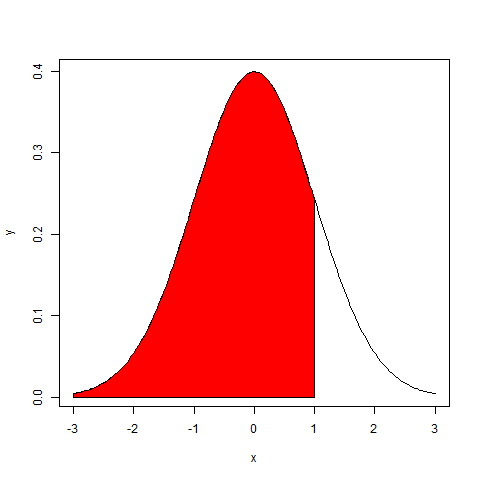
\includegraphics[width=0.45\linewidth]{image/fdistribuicao} 

}

\caption{Função distribuição N(x)}\label{fig:fdistribuicao}
\end{figure}
\centering

Fonte: Elaboração própria.

\justifying
\bigskip

O parâmetro da volatilidade não é um parâmetro que se consiga obter ou observar directamente, sendo um valor que representa a volatilidade esperada pelos investidores no futuro, conhecido como \textbf{volatilidade implícita}. Um modo de obter este valor é a partir dos restantes parâmetros, ou seja, tendo o valor de uma opção de compra, e considerando os valores de S\textsubscript{0}, K, r e T, substituir estes pelos respectivos valores e obter o valor de \(\sigma\) que iguale o valor da \emph{call} utilizando as equações \eqref{eq:call} e \eqref{eq:d1} através de processos por aproximação iterativo.

A volatilidade implícita será diferente consoante o preço de exercício da opção, considerando todos os outros parâmetros iguais. Da conjugação dos valore de volatilidade obtidos para cada um dos preços de exercício da opção obtêm-se um gráfico conhecido como \emph{volatility smile}(figura \ref{fig:volatilitysmile}). Este gráfico será o mesmo, quer se esteja a considerar uma opção do tipo \emph{call} ou a mesma equivalente opção do tipo \emph{put}.

\bigskip
\begin{figure}

{\centering 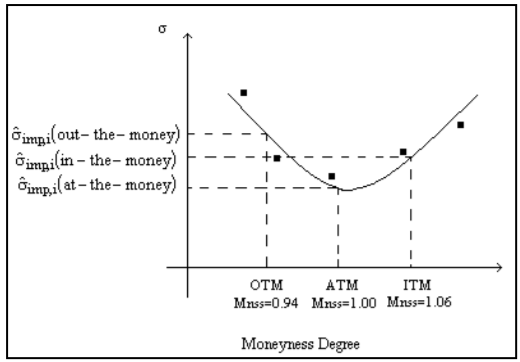
\includegraphics[width=0.6\linewidth]{image/volatilitysmile} 

}

\caption{Volatility Smile}\label{fig:volatilitysmile}
\end{figure}
\centering

Fonte: \citep[pp.182]{volatilitysmile}

\justifying
\bigskip

Como de pode ver pela figura \ref{fig:volatilitysmile} a opção é considerada \emph{out-the-money} se o seu valor for inferior ao do respectivo subjacente, \emph{at-the-money} se for superior e \emph{in-the-money} se o valor for igual. No calculo do valor da volatilidade será utilizado o valor de preço de exercício \emph{in-the-money} de opções do tipo \emph{call}, ou na impossibilidade do valor do subjacente ser o mesmo do K, o mais próximo deste.

Quando comparado com outros métodos para calcular a volatilidade onde os dados utilizados são dados históricos, este método incorpora o sentimento presente dos investidores relativo a volatilidade futura de um determinado ativo ou instrumento financeiro.

\hypertarget{portfolios-muxe9dia-variuxe2ncia}{%
\section{Portfolios média-variância}\label{portfolios-muxe9dia-variuxe2ncia}}

A otimização de portfolios através da diversificação é um conceito básico que teve origem em Markowitz, criando o conceito de fronteira eficiente. Existem vários pressupostos definidos na obtenção deste modelo, não sendo, no entanto, o âmbito aqui analisar esses mesmos pressupostos, considerando que independentemente disso esses mesmos pressupostos são verificados. De acordo com \citet{Modern2013}, ``todas os pressupostos acerca da analise de portfolio foram demonstradas serem simplistas, e em alguns casos demasiado simplistas.{[}\ldots{]}Pessoas necessitam apenas de se comportar como se fossem descritas pelos pressupostos para uma teoria ser válida'' \citep[pp.5]{Modern2013}.

Para aplicação deste modelo deve-se obter os seguintes dados dos instrumentos financeiros que vão constituir o portfolio:

\begin{itemize}
\tightlist
\item
  A taxa do retorno esperado, E(r);
\item
  O desvio padrão dos retornos, \(\sigma\);
\item
  O coeficiente de correlação,\(\rho\), entre cada um dos activos.
\end{itemize}

O retorno esperado vai depender de vários factores, essencialmente a taxa de retorno sem risco que se verifica no mercado, a taxa de inflação e o risco a que o investidor estará sujeito, sendo que quanto maior o risco, maior será o retorno esperado.
As séries dos retornos diários para cada um dos activos é calculada de acordo com a seguinte formula:

\begin{equation} 
  R_i = ln\Big(\frac{V_f}{V_i}\Big)
  \label{eq:logRet}
\end{equation}

A média dos retornos de cada um dos activos é calculada de acordo com a sua média aritmética:

\begin{equation} 
  \overline{R} = \frac{\displaystyle\sum_{i=1}^n R_i}{n}
  \label{eq:meanRet}
\end{equation}

O desvio padrão representa a volatilidade, ou risco, associada ao activo. Considerando que essa volatilidade é calculada com base nos dados históricos e as formulas acima, então a estatística da amostra para o desvio padrão representa-se pela seguinte formulas:

\begin{equation} 
  \hat{\sigma} = \sqrt\frac{\displaystyle\sum_{i=1}^n (R_i-\overline{R})^2}{n-1}
  \label{eq:estdesviopadrao}
\end{equation}

A escolha do tamanho da amostra (n) deve ser grande o suficiente de modo a garantir uma melhor precisão nas estatísticas obtidas, sendo que neste caso devemos considerar que a volatilidade não é constante ao longo do tempo e que valores mais antigos podem não ser tão relevantes como os valores mais recentes. De acordo com \citep{Hull2018} esse valor deve ser compreendido entre 90 a 180 dias para a cotação de activos.

Para o calculo da volatilidade anual utiliza-se os número de dias de negociação, sendo considerado 252 dias por ano como valor de referência.

\hypertarget{value-at-risk}{%
\section{Value at Risk}\label{value-at-risk}}

A quantificação do risco é fundamental para a gestão e atenuação de perdas no valor da carteira ao longo do tempo. Na gestão da carteira a aplicação de métricas de risco permite a adaptação contínua do portfólio aos fatores de risco quantificáveis, podendo-se, através de uma gestão ativa, manter o investidor devidamente informado relativamente ao risco que o seu investimento incorpora e poder tomar medidas proactivas de adaptação do investimento ao nível de risco verificado, tendo em consideração o perfil do investidor.O Value at Risk (VaR) é uma dessas métricas de risco.

O Value at Risk (VaR)\footnote{Markowitz foi dos primeiros autores a contemplar a análise de risco em investimentos, como se pode verificar em \citet{Markowitz1952}} é uma medida probabilística para a perda máxima provável de uma carteira para um nível de confiança determinado,num horizonte temporal especificado. Pode-se definir o VaR como ``descrevendo o quantil da distribuição de ganhos e perdas projectado ao longo do horizonte alvo. Se \emph{c} for o intervalo de confiança selecionado, VaR corresponde ao nível inferior da cauda 1-\emph{c}''\citep[pp.17]{philippe}. Este valor é sempre positivo.

O calculo do valor do VaR é de carácter obrigatório para entidades financeiras e seguradoras, sendo que os reguladores, dependendo da sua jurisdição, determinam os parâmetros quantitativos a serem utilizados.
No caso do Banco Central Europeu\footnote{ver relatório técnico \citet{ecb}}, esses parâmetros são de que o cálculo deve ser efectuado para um intervalo temporal de 10 dias de negociação e para um intervalo de confiança de 99\%, sendo considerado para esses cálculos pelo menos 250 dias negociação de observação de valores históricos.

O cálculo do VaR pode ser realizado de modos diferentes, existindo vários métodos, sendo considerados métodos de tipo não paramétrico, como o método histórico em que não se assume nenhum pressuposto na distribuição desses dados, ou métodos do tipo paramétrico, onde se assume um determinado tipo de distribuição dos dados. Para efeito desta dissertação será aplicado um método paramétrico para cálculo do VaR.

\hypertarget{var-paramuxe9trico-gaussiana}{%
\subsection{VaR Paramétrico (Gaussiana)}\label{var-paramuxe9trico-gaussiana}}

O VaR paramétrico pressupõe que os retornos diários apresentem uma distribuição normal (figura \ref{fig:var}), sendo que a sua representação matemática se encontra definida na equação \eqref{eq:var}.
\begin{equation} 
  VaR_{t+1}^{p} = -\sigma_{t+1}\Phi_{p}^{-1}
  \label{eq:var}
\end{equation}


\begin{figure}

{\centering 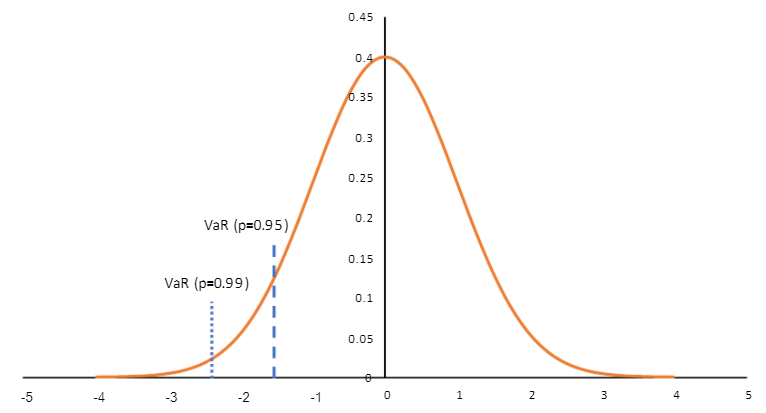
\includegraphics[width=0.6\linewidth]{image/VaR} 

}

\caption{VaR com intervalo confiança 95\% e 99\%.}\label{fig:var}
\end{figure}
\FloatBarrier
\centering

Fonte: \citep[pp.13]{phdthesis}

\justifying
\bigskip

O \(\Phi (p)\) representa a função distribuição e \(\Phi^{-1} (p)\) a sua inversa, sendo que, por exemplo, para um intervalo de confiança de 99\% o valor de \(\Phi^{-1} (p)\) corresponde a -2.33. Se considerarmos que a volatilidade prevista a 1 dia é de 2\%, teremos um VaR = -0.020*(-2.33), o que corresponde a um valor de 0.0466. Podemos interpretar o VaR como sendo a existência de 1\% de probabilidade de perder mais do que 4.66\% do valor investido no activo no dia de hoje.

O \emph{Daily Value at Risk} (DEaR) é o valor diariamente em risco, sendo calculado de acordo com a equação \eqref{eq:dear}.
\begin{equation} 
  €DEaR = € \textnormal{Valor de mercado do investimento} * VaR
  \label{eq:dear}  
\end{equation}

O valor do VaR a mais de um dia pode-se calcular a partir do DEaR a um dia, de acordo com a equação \eqref{eq:vardays}, onde N representa o número de dias.
\begin{equation} 
  VaR = DEaR*\sqrt{N}
  \label{eq:vardays}
\end{equation}

Se estivermos a analisar o VaR de um portfolio, esse é calculado da mesma forma que a variância de um portfolio (equação \eqref{eq:varport}), considerando o DEaR individual de cada componente.
\begin{equation} 
  DEaR_{portfolio} = \sum_{i=1}^{N}\sum_{j=1}^{N}Cov(DEaR_i,DEaR_j)
  \label{eq:varport}
\end{equation}
onde
\begin{equation} 
  Cov(DEaR_i,DEaR_j) = DEaR_{i}DEaR_{j}\rho(DEaR_i,DEaR_j)
  \label{eq:covport}
\end{equation}

Por exemplo, considerando 2 activos, A e B, constituintes de um portfolio, teríamos:
\begin{equation} 
  DEaR_{A+B}^{2} = DEar_{A}^{2}+DEaR_{B}^{2}+2\rho_{AB} DEaR_{A} DEaR_B
  \label{eq:ab}
\end{equation}

\hypertarget{var-paramuxe9trico-aproximauxe7uxe3o-cornish-fisher}{%
\subsection{VaR Paramétrico (Aproximação Cornish-Fisher)}\label{var-paramuxe9trico-aproximauxe7uxe3o-cornish-fisher}}

Quando a distribuição dos retornos apresentam excesso de curtose\footnote{medida de dispersão que caracteriza o achatamento da curva da função de distribuição} (\emph{Kurtosis}) e/ou assimetria\footnote{permite distinguir as distribuições assimétricas} (\emph{Skewness}) relativamente a uma distribuição normal pode-se proceder à aproximação Cornish-Fisher, permitindo desta forma uma aproximação ao VaR. Por exemplo, na figura \ref{fig:quant} temos uma distribuição do tipo leptocúrtica, sendo caracterizada por um pico mais alto e caudas mais pesadas que uma distribuição normal.
\bigskip

\begin{figure}

{\centering 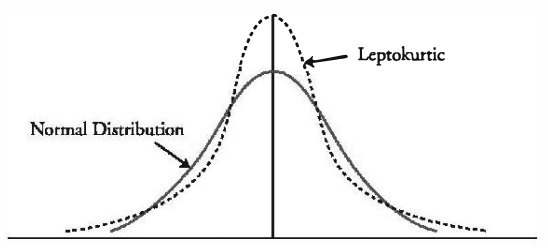
\includegraphics[width=0.6\linewidth]{image/kurtosis} 

}

\caption{Kurtosis}\label{fig:quant}
\end{figure}
\centering

Fonte: \citep[pp.46]{quant}

\justifying

O cálculo do VaR com aproximação Cornish-Fisher efectua-se de acordo com a equação \eqref{eq:varcf}, sendo que para calcular o valor referente a CF se aplica a equação \eqref{eq:cf}.
\begin{equation} 
  VaR_{t+1}^{p} = -\sigma_{t+1}*CF_{p}^{-1}
  \label{eq:varcf}
\end{equation}
onde
\begin{equation} 
  CF_{p}^{-1} = \Phi_{p}^{-1} + \frac{\zeta_{1}}{6}[(\Phi_{p}^{-1})^2-1] + \frac{\zeta_{2}}{24}[(\Phi_{p}^{-1})^3-3\Phi_{p}^{-1}] - \frac{\zeta_{1}^{2}}{36}[2(\Phi_{p}^{-1})^3-5\Phi_{p}^{-1}]
  \label{eq:cf}
\end{equation}

Os parâmetros referentes a \(\zeta_1\) e \(\zeta_2\) são respectivamente os valores da assimetria e do excesso de curtose. Esses valores são obtidos de acordo com as equações \eqref{eq:assimetria} e \eqref{eq:curtose}.
\begin{equation} 
 \zeta_1 = \frac{1}{n}\sum\bigg[\frac{X_i - \overline{X}}{\sigma}\bigg]^3
  \label{eq:assimetria}
\end{equation}
\begin{equation} 
 \zeta_2 = \frac{1}{n}\sum\bigg[\frac{X_i - \overline{X}}{\sigma}\bigg]^4 - 3
  \label{eq:curtose}
\end{equation}

\hypertarget{pacotes-do-r-para-anuxe1lise}{%
\chapter{Pacotes do R para análise}\label{pacotes-do-r-para-anuxe1lise}}

\newpage

We describe our methods in this chapter.

\hypertarget{aplicauxe7uxe3o-a-dados-do-modelo}{%
\chapter{Aplicação a dados do modelo}\label{aplicauxe7uxe3o-a-dados-do-modelo}}

\endgroup
\newpage

\hypertarget{aplicauxe7uxe3o-a-dados-do-modelo-1}{%
\section{Aplicação a dados do modelo}\label{aplicauxe7uxe3o-a-dados-do-modelo-1}}

A primeira fase consiste em extrair de forma aleatória 14 acções constituintes do Euro Stoxx 50, estando os valores obtidos representados na tabela \ref{tab:nice-tab}.
\scriptsize

\begin{table}[!h]

\caption{\label{tab:nice-tab}Empresas extraidas do Euro Stoxx 50}
\centering
\begin{tabular}[t]{l}
\toprule
x\\
\midrule
UNILEVER ORD\\
SOCIETE GENERALE ORD\\
BAYER N ORD\\
TELEFONICA ORD\\
ENEL ORD\\
\addlinespace
DEUTSCHE TELEKOM N ORD\\
AB INBEV ORD\\
DAIMLER N ORD\\
ORANGE ORD\\
SANOFI ORD\\
\addlinespace
AIRBUS ORD\\
INTESA SANPAOLO ORD\\
AHOLD DEL ORD\\
ASML HOLDING ORD\\
\bottomrule
\end{tabular}
\end{table}

\normalsize

Reference a figure by its code chunk label with the \texttt{fig:} prefix, e.g., see Figure \ref{fig:nice-fig}.
\scriptsize

\begin{figure}

{\centering \includegraphics[width=0.3\linewidth]{bookdown-demo_files/figure-latex/nice-fig-1} 

}

\caption{Here is a nice figure!}\label{fig:nice-fig}
\end{figure}

Calculo do retorno diario logaritmico
\scriptsize

\normalsize

Correlação entre activos
\scriptsize

\begin{Shaded}
\begin{Highlighting}[]
\CommentTok{\#do not print hash}
\CommentTok{\#options(width = 70)}
\CommentTok{\#cor(returns)}
\end{Highlighting}
\end{Shaded}

\normalsize

\scriptsize

\begin{Shaded}
\begin{Highlighting}[]
\CommentTok{\#par(mar = c(1,1,1,1))}
\CommentTok{\#plot(returns$TELEFONICA, main = "TEF.MC",col="red")}
\CommentTok{\#plot(returns$UNILEVER, main = "UNA.AS",col="red")}
\CommentTok{\#plot(returns$SOCGEN, main = "GLE.PA",col="red")}
\CommentTok{\#plot(returns$BAYER, main = "ENEL.MI",col="red")}
\CommentTok{\#plot(returns$ENEL, main = "BAYN.DE",col="red")}
\CommentTok{\#plot(returns$\textasciigrave{}DEUTSCHE TELEKOM\textasciigrave{}, main = "DTE.DE",col="red")}
\CommentTok{\#plot(returns$\textasciigrave{}AB INBEV\textasciigrave{}, main = "ABI.BR",col="red")}
\CommentTok{\#plot(returns$DAIMLER, main = "DAI.DE",col="red")}
\CommentTok{\#plot(returns$ORANGE, main = "ORA.PA",col="red")}
\CommentTok{\#plot(returns$SANOFI, main = "SAN.PA",col="red")}
\CommentTok{\#plot(returns$AIRBUS, main = "AIR.PA",col="red")}
\CommentTok{\#plot(returns$INTESA, main = "ISP.MI",col="red")}
\CommentTok{\#plot(returns$AHOLD, main = "AD.AS",col="red")}
\CommentTok{\#plot(returns$ASML, main = "ASML.AS",col="red")}
\end{Highlighting}
\end{Shaded}

\normalsize

\scriptsize

\begin{Shaded}
\begin{Highlighting}[]
 \CommentTok{\#par(mar = c(2,2,2,2))}
 \CommentTok{\#hist(returns$TELEFONICA,probability=T, main="TELEFONICA {-} daily.}
      \CommentTok{\#returns",xlab="Approximately normally distributed data",breaks=100)}
 \CommentTok{\#lines(density(na.omit(returns$TELEFONICA)),col=2)}
 \CommentTok{\#curve(dnorm(x,0,0.01640906), from = {-}0.15,to=0.15, col=\textquotesingle{}blue\textquotesingle{},add = TRUE)}
 \CommentTok{\#qqnorm(returns$TELEFONICA,main="QQ plot of normal data",pch=19)}
 \CommentTok{\#qqline(returns$TELEFONICA)}

\NormalTok{return\textless{}{-}return[}\OperatorTok{{-}}\DecValTok{1}\NormalTok{]}
\KeywordTok{hist}\NormalTok{(return,}\DataTypeTok{breaks=}\DecValTok{100}\NormalTok{)}
\KeywordTok{chart.Histogram}\NormalTok{(return,}\DataTypeTok{methods =} \KeywordTok{c}\NormalTok{(}\StringTok{"add.density"}\NormalTok{,}\StringTok{"add.normal"}\NormalTok{),}\DataTypeTok{colorset =} \KeywordTok{c}\NormalTok{(}\StringTok{"blue"}\NormalTok{,}\StringTok{"green"}\NormalTok{,}\StringTok{"red"}\NormalTok{))}
\KeywordTok{chartSeries}\NormalTok{(return,}\DataTypeTok{theme=}\StringTok{"white"}\NormalTok{)}
\end{Highlighting}
\end{Shaded}

\begin{center}\includegraphics[width=0.3\linewidth]{bookdown-demo_files/figure-latex/unnamed-chunk-7-1} \includegraphics[width=0.3\linewidth]{bookdown-demo_files/figure-latex/unnamed-chunk-7-2} \includegraphics[width=0.3\linewidth]{bookdown-demo_files/figure-latex/unnamed-chunk-7-3} \end{center}
\normalsize

\scriptsize

\begin{Shaded}
\begin{Highlighting}[]
 \CommentTok{\#TELTestNOR \textless{}{-} shapiro.test(as.numeric(returns$TELEFONICA))}
 \CommentTok{\#TELSha \textless{}{-} matrix(c(TELTestNOR$statistic,TELTestNOR$p.value),ncol = 2)}
 \CommentTok{\#colnames(TELSha) \textless{}{-} c("Estatistica","p{-}value")}
 \CommentTok{\#rownames(TELSha) \textless{}{-} c("Shapiro{-}Wilk normality test")}
 \CommentTok{\#TELSha \textless{}{-} as.table(TELSha)}
 \CommentTok{\#d \textless{}{-} knitr::kable(}
  \CommentTok{\#TELSha, caption = \textquotesingle{}Empresas extraidas do Euro Stoxx 50\textquotesingle{},}
  \CommentTok{\#booktabs = TRUE}
\CommentTok{\#)}
\CommentTok{\#kable\_styling(d, latex\_options = "hold\_position", position = "center")}
\end{Highlighting}
\end{Shaded}

\normalsize

Annualized volatility
\scriptsize

\normalsize

Como se pode verificar, o desvio padrão da empresa telecomunicação ``Telefonica'' é

sGARCH model with contant mean

\begin{Shaded}
\begin{Highlighting}[]
\NormalTok{s\textless{}{-}}\KeywordTok{ugarchspec}\NormalTok{(}\DataTypeTok{mean.model =} \KeywordTok{list}\NormalTok{(}\DataTypeTok{armaOrder=}\KeywordTok{c}\NormalTok{(}\DecValTok{0}\NormalTok{,}\DecValTok{0}\NormalTok{)),}\DataTypeTok{variance.model =} \KeywordTok{list}\NormalTok{(}\DataTypeTok{model=}\StringTok{"sGARCH"}\NormalTok{),}
              \DataTypeTok{distribution.model =} \StringTok{"norm"}\NormalTok{)}
\NormalTok{m\textless{}{-}}\KeywordTok{ugarchfit}\NormalTok{(}\DataTypeTok{data=}\NormalTok{return,}\DataTypeTok{spec=}\NormalTok{s)}
\NormalTok{m}
\end{Highlighting}
\end{Shaded}

\begin{verbatim}
## 
## *---------------------------------*
## *          GARCH Model Fit        *
## *---------------------------------*
## 
## Conditional Variance Dynamics    
## -----------------------------------
## GARCH Model  : sGARCH(1,1)
## Mean Model   : ARFIMA(0,0,0)
## Distribution : norm 
## 
## Optimal Parameters
## ------------------------------------
##         Estimate  Std. Error  t value Pr(>|t|)
## mu      0.000389    0.000392  0.99187  0.32126
## omega   0.000004    0.000002  1.71328  0.08666
## alpha1  0.075375    0.010477  7.19431  0.00000
## beta1   0.922271    0.010824 85.20606  0.00000
## 
## Robust Standard Errors:
##         Estimate  Std. Error  t value Pr(>|t|)
## mu      0.000389    0.000419  0.92904 0.352871
## omega   0.000004    0.000009  0.46954 0.638681
## alpha1  0.075375    0.035773  2.10704 0.035115
## beta1   0.922271    0.039301 23.46692 0.000000
## 
## LogLikelihood : 5059.169 
## 
## Information Criteria
## ------------------------------------
##                     
## Akaike       -4.9805
## Bayes        -4.9694
## Shibata      -4.9805
## Hannan-Quinn -4.9764
## 
## Weighted Ljung-Box Test on Standardized Residuals
## ------------------------------------
##                         statistic   p-value
## Lag[1]                      11.48 0.0007035
## Lag[2*(p+q)+(p+q)-1][2]     11.73 0.0006672
## Lag[4*(p+q)+(p+q)-1][5]     12.13 0.0025719
## d.o.f=0
## H0 : No serial correlation
## 
## Weighted Ljung-Box Test on Standardized Squared Residuals
## ------------------------------------
##                         statistic p-value
## Lag[1]                      1.074  0.3001
## Lag[2*(p+q)+(p+q)-1][5]     2.189  0.5744
## Lag[4*(p+q)+(p+q)-1][9]     3.741  0.6330
## d.o.f=2
## 
## Weighted ARCH LM Tests
## ------------------------------------
##             Statistic Shape Scale P-Value
## ARCH Lag[3]   0.08693 0.500 2.000  0.7681
## ARCH Lag[5]   2.35507 1.440 1.667  0.3980
## ARCH Lag[7]   3.09298 2.315 1.543  0.4962
## 
## Nyblom stability test
## ------------------------------------
## Joint Statistic:  1.4582
## Individual Statistics:              
## mu     0.42569
## omega  0.24745
## alpha1 0.11803
## beta1  0.06953
## 
## Asymptotic Critical Values (10% 5% 1%)
## Joint Statistic:          1.07 1.24 1.6
## Individual Statistic:     0.35 0.47 0.75
## 
## Sign Bias Test
## ------------------------------------
##                    t-value   prob sig
## Sign Bias           0.3640 0.7159    
## Negative Sign Bias  1.2678 0.2050    
## Positive Sign Bias  0.7081 0.4790    
## Joint Effect        2.1270 0.5465    
## 
## 
## Adjusted Pearson Goodness-of-Fit Test:
## ------------------------------------
##   group statistic p-value(g-1)
## 1    20     71.95    4.346e-08
## 2    30    103.28    2.901e-10
## 3    40     97.57    6.354e-07
## 4    50    115.42    2.788e-07
## 
## 
## Elapsed time : 0.180541
\end{verbatim}

\begin{Shaded}
\begin{Highlighting}[]
\KeywordTok{plot}\NormalTok{(m,}\DataTypeTok{which =} \StringTok{"all"}\NormalTok{)}
\end{Highlighting}
\end{Shaded}

\begin{verbatim}
## 
## please wait...calculating quantiles...
\end{verbatim}

\begin{Shaded}
\begin{Highlighting}[]
\NormalTok{f\textless{}{-}}\KeywordTok{ugarchforecast}\NormalTok{(}\DataTypeTok{fitORspec =}\NormalTok{ m,}\DataTypeTok{n.ahead =} \DecValTok{60}\NormalTok{)}
\KeywordTok{plot}\NormalTok{(}\KeywordTok{fitted}\NormalTok{(f))}
\KeywordTok{plot}\NormalTok{(}\KeywordTok{sigma}\NormalTok{(f))}
\end{Highlighting}
\end{Shaded}

\begin{center}\includegraphics{bookdown-demo_files/figure-latex/unnamed-chunk-10-1} \includegraphics{bookdown-demo_files/figure-latex/unnamed-chunk-10-2} \includegraphics{bookdown-demo_files/figure-latex/unnamed-chunk-10-3} \end{center}

Application example - potfolio allocation

\begin{Shaded}
\begin{Highlighting}[]
\NormalTok{v\textless{}{-}}\KeywordTok{sqrt}\NormalTok{(}\DecValTok{252}\NormalTok{)}\OperatorTok{*}\KeywordTok{sigma}\NormalTok{(m)}
\NormalTok{w\textless{}{-}}\FloatTok{0.05}\OperatorTok{/}\NormalTok{v}
\KeywordTok{plot}\NormalTok{(}\KeywordTok{merge}\NormalTok{(v,w),}\DataTypeTok{multi.panel=}\OtherTok{TRUE}\NormalTok{)}
\end{Highlighting}
\end{Shaded}

\begin{center}\includegraphics{bookdown-demo_files/figure-latex/unnamed-chunk-11-1} \end{center}

GARCH with sstd

\begin{Shaded}
\begin{Highlighting}[]
\NormalTok{s\textless{}{-}}\KeywordTok{ugarchspec}\NormalTok{(}\DataTypeTok{mean.model =} \KeywordTok{list}\NormalTok{(}\DataTypeTok{armaOrder=}\KeywordTok{c}\NormalTok{(}\DecValTok{0}\NormalTok{,}\DecValTok{0}\NormalTok{)),}\DataTypeTok{variance.model =} \KeywordTok{list}\NormalTok{(}\DataTypeTok{model=}\StringTok{"sGARCH"}\NormalTok{),}
              \DataTypeTok{distribution.model =} \StringTok{"sstd"}\NormalTok{)}
\NormalTok{m\textless{}{-}}\KeywordTok{ugarchfit}\NormalTok{(}\DataTypeTok{data=}\NormalTok{return,}\DataTypeTok{spec=}\NormalTok{s)}
\NormalTok{m}
\end{Highlighting}
\end{Shaded}

\begin{verbatim}
## 
## *---------------------------------*
## *          GARCH Model Fit        *
## *---------------------------------*
## 
## Conditional Variance Dynamics    
## -----------------------------------
## GARCH Model  : sGARCH(1,1)
## Mean Model   : ARFIMA(0,0,0)
## Distribution : sstd 
## 
## Optimal Parameters
## ------------------------------------
##         Estimate  Std. Error  t value Pr(>|t|)
## mu      0.000255    0.000391  0.65304 0.513731
## omega   0.000005    0.000004  1.36064 0.173627
## alpha1  0.064102    0.013708  4.67619 0.000003
## beta1   0.929022    0.015711 59.13126 0.000000
## skew    1.019436    0.031535 32.32671 0.000000
## shape   5.178852    0.573798  9.02557 0.000000
## 
## Robust Standard Errors:
##         Estimate  Std. Error  t value Pr(>|t|)
## mu      0.000255    0.000402  0.63445 0.525784
## omega   0.000005    0.000009  0.53828 0.590383
## alpha1  0.064102    0.031607  2.02807 0.042553
## beta1   0.929022    0.038615 24.05869 0.000000
## skew    1.019436    0.028874 35.30686 0.000000
## shape   5.178852    0.637241  8.12699 0.000000
## 
## LogLikelihood : 5153.861 
## 
## Information Criteria
## ------------------------------------
##                     
## Akaike       -5.0718
## Bayes        -5.0552
## Shibata      -5.0718
## Hannan-Quinn -5.0657
## 
## Weighted Ljung-Box Test on Standardized Residuals
## ------------------------------------
##                         statistic   p-value
## Lag[1]                      10.87 0.0009800
## Lag[2*(p+q)+(p+q)-1][2]     11.16 0.0009447
## Lag[4*(p+q)+(p+q)-1][5]     11.63 0.0034717
## d.o.f=0
## H0 : No serial correlation
## 
## Weighted Ljung-Box Test on Standardized Squared Residuals
## ------------------------------------
##                         statistic p-value
## Lag[1]                      1.989  0.1584
## Lag[2*(p+q)+(p+q)-1][5]     2.966  0.4133
## Lag[4*(p+q)+(p+q)-1][9]     5.037  0.4241
## d.o.f=2
## 
## Weighted ARCH LM Tests
## ------------------------------------
##             Statistic Shape Scale P-Value
## ARCH Lag[3]  0.006045 0.500 2.000  0.9380
## ARCH Lag[5]  2.652356 1.440 1.667  0.3443
## ARCH Lag[7]  3.804502 2.315 1.543  0.3756
## 
## Nyblom stability test
## ------------------------------------
## Joint Statistic:  3.5779
## Individual Statistics:              
## mu     0.27077
## omega  0.36609
## alpha1 0.20932
## beta1  0.40154
## skew   0.04104
## shape  0.54690
## 
## Asymptotic Critical Values (10% 5% 1%)
## Joint Statistic:          1.49 1.68 2.12
## Individual Statistic:     0.35 0.47 0.75
## 
## Sign Bias Test
## ------------------------------------
##                    t-value   prob sig
## Sign Bias           0.3186 0.7500    
## Negative Sign Bias  1.6346 0.1023    
## Positive Sign Bias  1.1215 0.2622    
## Joint Effect        3.9400 0.2680    
## 
## 
## Adjusted Pearson Goodness-of-Fit Test:
## ------------------------------------
##   group statistic p-value(g-1)
## 1    20     27.79      0.08749
## 2    30     32.17      0.31257
## 3    40     55.16      0.04474
## 4    50     49.75      0.44312
## 
## 
## Elapsed time : 0.773948
\end{verbatim}

\begin{Shaded}
\begin{Highlighting}[]
\KeywordTok{plot}\NormalTok{(m,}\DataTypeTok{which =} \StringTok{"all"}\NormalTok{)}
\end{Highlighting}
\end{Shaded}

\begin{verbatim}
## 
## please wait...calculating quantiles...
\end{verbatim}

\begin{Shaded}
\begin{Highlighting}[]
\NormalTok{f\textless{}{-}}\KeywordTok{ugarchforecast}\NormalTok{(}\DataTypeTok{fitORspec =}\NormalTok{ m,}\DataTypeTok{n.ahead =} \DecValTok{60}\NormalTok{)}
\KeywordTok{plot}\NormalTok{(}\KeywordTok{fitted}\NormalTok{(f))}
\KeywordTok{plot}\NormalTok{(}\KeywordTok{sigma}\NormalTok{(f))}
\end{Highlighting}
\end{Shaded}

\begin{center}\includegraphics{bookdown-demo_files/figure-latex/unnamed-chunk-12-1} \includegraphics{bookdown-demo_files/figure-latex/unnamed-chunk-12-2} \includegraphics{bookdown-demo_files/figure-latex/unnamed-chunk-12-3} \end{center}

GJR-GARCH

\begin{Shaded}
\begin{Highlighting}[]
\NormalTok{s\textless{}{-}}\KeywordTok{ugarchspec}\NormalTok{(}\DataTypeTok{mean.model =} \KeywordTok{list}\NormalTok{(}\DataTypeTok{armaOrder=}\KeywordTok{c}\NormalTok{(}\DecValTok{0}\NormalTok{,}\DecValTok{0}\NormalTok{)),}\DataTypeTok{variance.model =} \KeywordTok{list}\NormalTok{(}\DataTypeTok{model=}\StringTok{"gjrGARCH"}\NormalTok{),}
              \DataTypeTok{distribution.model =} \StringTok{"sstd"}\NormalTok{)}
\NormalTok{m\textless{}{-}}\KeywordTok{ugarchfit}\NormalTok{(}\DataTypeTok{data=}\NormalTok{return,}\DataTypeTok{spec=}\NormalTok{s)}
\NormalTok{m}
\end{Highlighting}
\end{Shaded}

\begin{verbatim}
## 
## *---------------------------------*
## *          GARCH Model Fit        *
## *---------------------------------*
## 
## Conditional Variance Dynamics    
## -----------------------------------
## GARCH Model  : gjrGARCH(1,1)
## Mean Model   : ARFIMA(0,0,0)
## Distribution : sstd 
## 
## Optimal Parameters
## ------------------------------------
##         Estimate  Std. Error  t value Pr(>|t|)
## mu      0.000122    0.000388  0.31361 0.753820
## omega   0.000006    0.000004  1.39140 0.164104
## alpha1  0.029608    0.010561  2.80351 0.005055
## beta1   0.921084    0.015405 59.79096 0.000000
## gamma1  0.084912    0.023364  3.63435 0.000279
## skew    1.018822    0.031592 32.24906 0.000000
## shape   5.320881    0.598556  8.88952 0.000000
## 
## Robust Standard Errors:
##         Estimate  Std. Error  t value Pr(>|t|)
## mu      0.000122    0.000409  0.29715 0.766350
## omega   0.000006    0.000010  0.57529 0.565099
## alpha1  0.029608    0.011326  2.61409 0.008947
## beta1   0.921084    0.031316 29.41235 0.000000
## gamma1  0.084912    0.041527  2.04476 0.040878
## skew    1.018822    0.030441 33.46821 0.000000
## shape   5.320881    0.694823  7.65789 0.000000
## 
## LogLikelihood : 5164.008 
## 
## Information Criteria
## ------------------------------------
##                     
## Akaike       -5.0808
## Bayes        -5.0614
## Shibata      -5.0808
## Hannan-Quinn -5.0737
## 
## Weighted Ljung-Box Test on Standardized Residuals
## ------------------------------------
##                         statistic  p-value
## Lag[1]                      10.79 0.001022
## Lag[2*(p+q)+(p+q)-1][2]     11.01 0.001035
## Lag[4*(p+q)+(p+q)-1][5]     11.34 0.004136
## d.o.f=0
## H0 : No serial correlation
## 
## Weighted Ljung-Box Test on Standardized Squared Residuals
## ------------------------------------
##                         statistic p-value
## Lag[1]                      1.161  0.2813
## Lag[2*(p+q)+(p+q)-1][5]     2.869  0.4315
## Lag[4*(p+q)+(p+q)-1][9]     4.165  0.5612
## d.o.f=2
## 
## Weighted ARCH LM Tests
## ------------------------------------
##             Statistic Shape Scale P-Value
## ARCH Lag[3]    0.5849 0.500 2.000  0.4444
## ARCH Lag[5]    2.4806 1.440 1.667  0.3745
## ARCH Lag[7]    2.9191 2.315 1.543  0.5290
## 
## Nyblom stability test
## ------------------------------------
## Joint Statistic:  2.3582
## Individual Statistics:              
## mu     0.56969
## omega  0.73784
## alpha1 0.57993
## beta1  0.87042
## gamma1 0.64879
## skew   0.02895
## shape  0.98210
## 
## Asymptotic Critical Values (10% 5% 1%)
## Joint Statistic:          1.69 1.9 2.35
## Individual Statistic:     0.35 0.47 0.75
## 
## Sign Bias Test
## ------------------------------------
##                    t-value   prob sig
## Sign Bias           0.2050 0.8376    
## Negative Sign Bias  0.4205 0.6741    
## Positive Sign Bias  1.5051 0.1324    
## Joint Effect        3.3281 0.3438    
## 
## 
## Adjusted Pearson Goodness-of-Fit Test:
## ------------------------------------
##   group statistic p-value(g-1)
## 1    20     15.81       0.6697
## 2    30     29.86       0.4209
## 3    40     40.94       0.3855
## 4    50     60.89       0.1187
## 
## 
## Elapsed time : 1.27297
\end{verbatim}

\begin{Shaded}
\begin{Highlighting}[]
\KeywordTok{plot}\NormalTok{(m,}\DataTypeTok{which =} \StringTok{"all"}\NormalTok{)}
\end{Highlighting}
\end{Shaded}

\begin{verbatim}
## 
## please wait...calculating quantiles...
\end{verbatim}

\begin{Shaded}
\begin{Highlighting}[]
\NormalTok{f\textless{}{-}}\KeywordTok{ugarchforecast}\NormalTok{(}\DataTypeTok{fitORspec =}\NormalTok{ m,}\DataTypeTok{n.ahead =} \DecValTok{60}\NormalTok{)}
\KeywordTok{plot}\NormalTok{(}\KeywordTok{fitted}\NormalTok{(f))}
\KeywordTok{plot}\NormalTok{(}\KeywordTok{sigma}\NormalTok{(f))}
\end{Highlighting}
\end{Shaded}

\begin{center}\includegraphics{bookdown-demo_files/figure-latex/unnamed-chunk-13-1} \includegraphics{bookdown-demo_files/figure-latex/unnamed-chunk-13-2} \includegraphics{bookdown-demo_files/figure-latex/unnamed-chunk-13-3} \end{center}

GJR-GARCH in mean

\begin{Shaded}
\begin{Highlighting}[]
\NormalTok{s\textless{}{-}}\KeywordTok{ugarchspec}\NormalTok{(}\DataTypeTok{mean.model =} \KeywordTok{list}\NormalTok{(}\DataTypeTok{armaOrder=}\KeywordTok{c}\NormalTok{(}\DecValTok{0}\NormalTok{,}\DecValTok{0}\NormalTok{),}\DataTypeTok{archm=}\NormalTok{T,}\DataTypeTok{archpow=}\DecValTok{2}\NormalTok{),}\DataTypeTok{variance.model =} \KeywordTok{list}\NormalTok{(}\DataTypeTok{model=}\StringTok{"sGARCH"}\NormalTok{)}
\NormalTok{              ,}\DataTypeTok{distribution.model =} \StringTok{"sstd"}\NormalTok{)}
\NormalTok{m\textless{}{-}}\KeywordTok{ugarchfit}\NormalTok{(}\DataTypeTok{data=}\NormalTok{return,}\DataTypeTok{spec=}\NormalTok{s)}
\NormalTok{m}
\end{Highlighting}
\end{Shaded}

\begin{verbatim}
## 
## *---------------------------------*
## *          GARCH Model Fit        *
## *---------------------------------*
## 
## Conditional Variance Dynamics    
## -----------------------------------
## GARCH Model  : sGARCH(1,1)
## Mean Model   : ARFIMA(0,0,0)
## Distribution : sstd 
## 
## Optimal Parameters
## ------------------------------------
##         Estimate  Std. Error  t value Pr(>|t|)
## mu     -0.000548    0.000561 -0.97667 0.328731
## archm   2.516780    1.267853  1.98507 0.047136
## omega   0.000005    0.000003  1.34986 0.177062
## alpha1  0.063407    0.013410  4.72831 0.000002
## beta1   0.930139    0.015162 61.34597 0.000000
## skew    1.026251    0.031792 32.28044 0.000000
## shape   5.145742    0.571638  9.00175 0.000000
## 
## Robust Standard Errors:
##         Estimate  Std. Error  t value Pr(>|t|)
## mu     -0.000548    0.000547 -1.00133 0.316667
## archm   2.516780    1.167343  2.15599 0.031084
## omega   0.000005    0.000009  0.53121 0.595276
## alpha1  0.063407    0.030464  2.08136 0.037401
## beta1   0.930139    0.036857 25.23623 0.000000
## skew    1.026251    0.029082 35.28832 0.000000
## shape   5.145742    0.648904  7.92990 0.000000
## 
## LogLikelihood : 5155.77 
## 
## Information Criteria
## ------------------------------------
##                     
## Akaike       -5.0727
## Bayes        -5.0533
## Shibata      -5.0727
## Hannan-Quinn -5.0656
## 
## Weighted Ljung-Box Test on Standardized Residuals
## ------------------------------------
##                         statistic  p-value
## Lag[1]                      10.74 0.001049
## Lag[2*(p+q)+(p+q)-1][2]     11.02 0.001027
## Lag[4*(p+q)+(p+q)-1][5]     11.48 0.003805
## d.o.f=0
## H0 : No serial correlation
## 
## Weighted Ljung-Box Test on Standardized Squared Residuals
## ------------------------------------
##                         statistic p-value
## Lag[1]                      2.069  0.1503
## Lag[2*(p+q)+(p+q)-1][5]     3.234  0.3660
## Lag[4*(p+q)+(p+q)-1][9]     5.495  0.3604
## d.o.f=2
## 
## Weighted ARCH LM Tests
## ------------------------------------
##             Statistic Shape Scale P-Value
## ARCH Lag[3]   0.05879 0.500 2.000  0.8084
## ARCH Lag[5]   3.18122 1.440 1.667  0.2646
## ARCH Lag[7]   4.31781 2.315 1.543  0.3031
## 
## Nyblom stability test
## ------------------------------------
## Joint Statistic:  4.0828
## Individual Statistics:              
## mu     0.11797
## archm  0.35490
## omega  0.41429
## alpha1 0.24075
## beta1  0.44941
## skew   0.06264
## shape  0.56250
## 
## Asymptotic Critical Values (10% 5% 1%)
## Joint Statistic:          1.69 1.9 2.35
## Individual Statistic:     0.35 0.47 0.75
## 
## Sign Bias Test
## ------------------------------------
##                    t-value   prob sig
## Sign Bias           0.4536 0.6502    
## Negative Sign Bias  1.5163 0.1296    
## Positive Sign Bias  1.0083 0.3134    
## Joint Effect        3.4130 0.3322    
## 
## 
## Adjusted Pearson Goodness-of-Fit Test:
## ------------------------------------
##   group statistic p-value(g-1)
## 1    20     25.37      0.14874
## 2    30     32.70      0.29002
## 3    40     45.82      0.21009
## 4    50     63.60      0.07853
## 
## 
## Elapsed time : 1.176525
\end{verbatim}

\begin{Shaded}
\begin{Highlighting}[]
\KeywordTok{plot}\NormalTok{(m,}\DataTypeTok{which =} \StringTok{"all"}\NormalTok{)}
\end{Highlighting}
\end{Shaded}

\begin{verbatim}
## 
## please wait...calculating quantiles...
\end{verbatim}

\begin{Shaded}
\begin{Highlighting}[]
\NormalTok{f\textless{}{-}}\KeywordTok{ugarchforecast}\NormalTok{(}\DataTypeTok{fitORspec =}\NormalTok{ m,}\DataTypeTok{n.ahead =} \DecValTok{60}\NormalTok{)}
\KeywordTok{plot}\NormalTok{(}\KeywordTok{fitted}\NormalTok{(f))}
\KeywordTok{plot}\NormalTok{(}\KeywordTok{sigma}\NormalTok{(f))}
\end{Highlighting}
\end{Shaded}

\begin{center}\includegraphics{bookdown-demo_files/figure-latex/unnamed-chunk-14-1} \includegraphics{bookdown-demo_files/figure-latex/unnamed-chunk-14-2} \includegraphics{bookdown-demo_files/figure-latex/unnamed-chunk-14-3} \end{center}

\hypertarget{conclusuxe3o}{%
\chapter*{Conclusão}\label{conclusuxe3o}}
\addcontentsline{toc}{chapter}{Conclusão}

We have finished a nice book.

  \bibliography{book.bib,packages.bib}

\part*{Apêndices}
\addcontentsline{toc}{part}{Apêndices}

\newpage
\part*{\normalfont\huge\bfseries\centering Apêndice I}
\newpage

\part*{\normalfont\huge\bfseries\centering Apêndice II}
\newpage

\end{document}
